\section{训练模型}
\label{sec:train-model}

\begin{frame}
  \begin{center}
    \Huge{\textcolor{red}{训练模型}}
  \end{center}

  \begin{enumerate}
    \item \alert{优化算法}
    \item \alert{工作流}
  \end{enumerate}    
\end{frame}

\subsection{优化算法}

\begin{frame}[fragile]{优化器}
  \begin{python} 
class Optimizer(object):
  """Add operations to minimize `loss` by updating `var\_list`.
  """
  def minimize(self, loss, var_list):
    grads_and_vars = self.compute_gradients(loss, var_list)
    return self.apply_gradients(grads_and_vars)
  \end{python}
\end{frame}

\begin{frame}[fragile]{计算梯度}
  \begin{python} 
def computea_gradients(loss, var_list):
  grads = gradients(loss, var_list, grad)
  return list(zip(grads, var_list))

def gradients(loss, var_list, grads=1):
  ops_and_grads = {}
  for op in reversed_graph(loss).topological_sort():
    grad = op.grad_fn(grad)
    ops_and_grads[op] = grad
  return [ops_and_grads.get(var) for var in var_list]
  \end{python}
\end{frame}

\begin{frame}[fragile]{梯度函数}
  \begin{python}
@ops.RegisterGradient("op_name")
def grad_func(op, grad):
  """construct gradient subgraph for an op type.
  Returns:
    A list of gradients, one per each input of `op`.
  """
  return cons_grad_subgraph(op, grad) 
  \end{python}

\[\begin{gathered}
  \left( {{y_1},{y_2},...,{y_m}} \right) = f\left( {{x_1},{x_2},...,{x_n}} \right) \hfill \\
  \left( {{\raise0.5ex\hbox{$\scriptstyle {\partial L}$}
\kern-0.1em/\kern-0.15em
\lower0.25ex\hbox{$\scriptstyle {\partial {x_1}}$}},{\raise0.5ex\hbox{$\scriptstyle {\partial L}$}
\kern-0.1em/\kern-0.15em
\lower0.25ex\hbox{$\scriptstyle {\partial {x_2}}$}},...,{\raise0.5ex\hbox{$\scriptstyle {\partial L}$}
\kern-0.1em/\kern-0.15em
\lower0.25ex\hbox{$\scriptstyle {\partial {x_n}}$}}} \right) = g\left( {{x_1},{x_2},...,{x_n};{\raise0.5ex\hbox{$\scriptstyle {\partial L}$}
\kern-0.1em/\kern-0.15em
\lower0.25ex\hbox{$\scriptstyle {\partial {y_1}}$}},{\raise0.5ex\hbox{$\scriptstyle {\partial L}$}
\kern-0.1em/\kern-0.15em
\lower0.25ex\hbox{$\scriptstyle {\partial {y_2}}$}},...,{\raise0.5ex\hbox{$\scriptstyle {\partial L}$}
\kern-0.1em/\kern-0.15em
\lower0.25ex\hbox{$\scriptstyle {\partial {y_n}}$}}} \right) \hfill \\
  \frac{{\partial L}}{{\partial {x_i}}} = \sum\limits_{j = 1}^m {\frac{{\partial L}}{{\partial {y_j}}}\frac{{\partial {y_j}}}{{\partial {x_i}}}} {\text{     for }}i = 1,2,...,n{\text{ }} \hfill \\ 
\end{gathered} \]
\end{frame}

\begin{frame}[fragile]{例子:SquareGrad函数}
  \begin{python}
@ops.RegisterGradient("Square")
def SquareGrad(op, grad):
  x = op.inputs[0]
  with ops.control_dependencies([grad.op]):
    return grad * (2.0 * x)
  \end{python}

  \begin{figure}
    \centering
    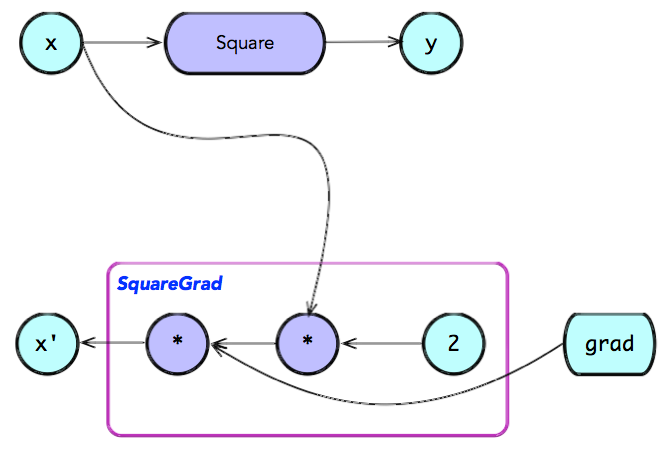
\includegraphics[width=0.55\textwidth]{square-grad.png}
  \end{figure}
\end{frame}

\begin{frame}[fragile]{应用梯度}
  \begin{python} 
def apply_gradients(grads_and_vars, learning_rate):
  for (grad, var) in grads_and_vars:
    apply_gradient_descent(learning_rate, grad, var)
  \end{python}
  \begin{figure}
    \centering
    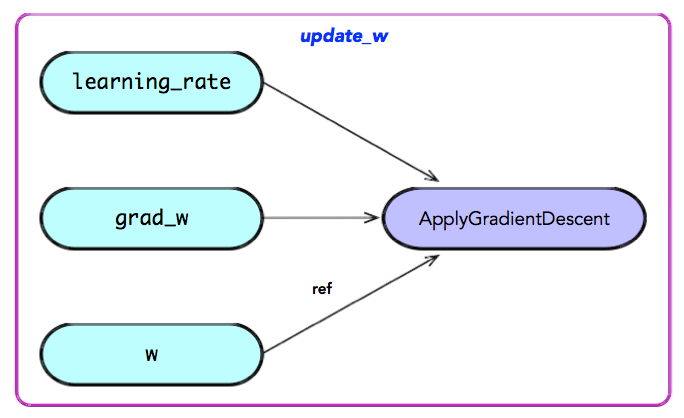
\includegraphics[width=0.6\textwidth]{apply-grad-w.png}
  \end{figure}  
\end{frame}

\begin{frame}{RunStep过程}
  \begin{figure}
    \centering
    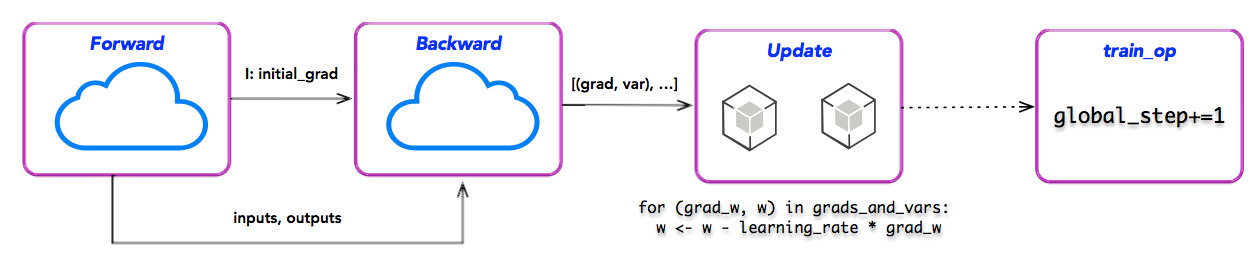
\includegraphics[width=1.0\textwidth]{bp-train-pipeline.png}
  \end{figure}
\end{frame}
